%%%%%%%%%%%%%%%%%%%%%%%%
%This tempelate is provided by Abdorrahman Mehri Ghahfarrokhi, petroleum university of technology, department of energy economics.
%email address: amehri.ghahfarrokhi@gmail.com
%%%%%%%%%%%%%%%%%%%%%%%%%

\RequirePackage[utf8]{inputenc}
\RequirePackage[T1]{fontenc}
\documentclass [xcolor=svgnames, t] {beamer} 
\usepackage[utf8]{inputenc}
\usepackage{booktabs, comment}
%\usepackage[slovak]{babel}
\usepackage[absolute, overlay]{textpos} 
\usepackage{pgfpages}
\usepackage[font=footnotesize]{caption}
\useoutertheme{infolines} 

\definecolor{red}{RGB}{250,0,75}
\setbeamercolor{title in head/foot}{bg=red, fg=white}
\setbeamercolor{author in head/foot}{bg=myuniversity}
\setbeamertemplate{page number in head/foot}{}
\usepackage{csquotes}


\usepackage{amsmath}
\usepackage[makeroom]{cancel}


\usepackage{textpos}

\usepackage{tikz}
\usepackage{algpseudocode}  % part of algorithmicx package
\usepackage{algorithm}

\usetheme{Madrid}
\definecolor{myuniversity}{RGB}{0, 85, 150}
\usecolortheme[named=myuniversity]{structure}
\usepackage{tikz}

\newtheorem{defn}{Definition}[section]
\newtheorem{thm}{Theorem}[section]
\newtheorem{claim}{Claim}[section]


\newtheorem{Shap}{Shapleyho hodnota}[section]
\newtheorem{Vektor}{\textbf{Vektorový prostor $\Gamma^n$}}[section]
\newtheorem{Trh}{Trh}[section]
\newtheorem{Obchod}{Obchod}[section]
\newtheorem{Volhra}{Volební hra}[section]

\newtheorem{Jednohlas}{\textbf{Shapleyho hodnota jednohlasných her}}[section]
\newtheorem{Jadro}{Jadro}[section]

\newtheorem{Lemke}{Lemke-Howson algorithm}[section]
\newtheorem{Nic}{}[section]
\def\QQ{\mathbb{Q}}
\def\RR{\mathbb{R}}
\def\ZZ{\mathbb{Z}}
\def\NN{\mathbb{N}}

\algnewcommand\algorithmicswitch{\textbf{switch}}
\algnewcommand\algorithmiccase{\textbf{case}}
\algnewcommand\algorithmicassert{\texttt{assert}}
\algnewcommand\Assert[1]{\State \algorithmicassert(#1)}%
% New "environments"
\algdef{SE}[SWITCH]{Switch}{EndSwitch}[1]{\algorithmicswitch\ #1\ \algorithmicdo}{\algorithmicend\ \algorithmicswitch}%
\algdef{SE}[CASE]{Case}{EndCase}[1]{\algorithmiccase\ #1}{\algorithmicend\ \algorithmiccase}%
\algtext*{EndSwitch}%
\algtext*{EndCase}%



\title[Generalized Logistic Problems]{Generalized Logistic Problems}
\institute[]{Pavol Jozef Šafárik University in Košice \\ Institute of Computer Science}
\titlegraphic{
\includegraphics[height=1.95cm]{picture/logopfupjsf.jpg}}
\author[Mgr. N. Micheľ]{
	\\ Mgr. Norbert Micheľ \\
    Supervisor:
    \\
    prof. RNDr. Gabriel Semanišin, PhD.
    }

\date{January 2026}

\addtobeamertemplate{navigation symbols}{}{%
    \usebeamerfont{footline}%
    \usebeamercolor[fg]{footline}%
    \hspace{1em}%
    \insertframenumber/\inserttotalframenumber
}

\begin{document}
\begin{frame}
\maketitle
\end{frame}

%%%%%%%%%%%%%%%%%%%%%%%%%%%%
%\logo{
\includegraphics[scale=0.14]{upjs-logo.png}}

%%%%%%%%%%%%%%%%%%%%%%%%%%

\begin{frame}
\frametitle{Contents}
\tableofcontents
\end{frame}

\begin{frame}{Cut-Path}


\begin{defn}[Cut-Path]
Let \(G = (V, E)\) be a graph, and let \(u, v \in V\) be two distinct vertices. A cut-path between \(u\) and \(v\) is a set of edges \(S \subseteq E\) such that:
\begin{itemize}
    \item There exist subsets \(A, B \subseteq S\) where:
    \begin{itemize}
        \item \(A\) is a cut separating \(u\) and \(v\) (i.e., removing \(A\) disconnects \(u\) and \(v\)),
        \item \(B\) is a path connecting \(u\) and \(v\) (i.e., \(B\) forms a sequence of edges between \(u\) and \(v\)).
    \end{itemize}
\end{itemize}
\end{defn}
\end{frame}



\begin{frame}{Notation}
\scriptsize
\begin{defn}[Value of Minimum Cut-Path]
Let \(G = (V, E)\) be a graph, and let \(u, v \in V\) be two distinct vertices. The minimum size of any cut-path between \(u\) and \(v\), denoted by \(\text{cp}(u, v)\), is defined as:
\[
\text{cp}(u, v) = \min\{ |S| \mid S \in \text{cut-path}(u, v) \}.
\]
\end{defn}

\begin{defn}[Distance]
Let \(G = (V, E)\) be a graph, and let \(u, v \in V\) be two distinct vertices. The distance between \(u\) and \(v\), denoted by \(d(u, v)\), is defined as the minimum number of edges in any path between \(u\) and \(v\). Formally:
\[
d(u, v) = \min\{ |P| \mid P \in path(u, v) \}.
\]
\end{defn}

\begin{defn}[Value of Minimum Cut]
Let \(G = (V, E)\) be a graph, and let \(u, v \in V\) be two distinct vertices. The value \(c(u, v)\) is defined as the minimum size of a cut between \(u\) and \(v\). Formally:
\[
c(u, v) = \min\{ |C| \mid C \in cut(u, v) \}.
\]
\end{defn}

\end{frame}


\section{$1^{st}$ article}


\begin{frame}{$1^{st}$ article}
\begin{itemize}
    \item \textbf{Min Cut-Path problem is NP-complete}
    \begin{itemize}
        \item NP-completeness proved via a two-step reduction from \textsc{3-SAT}
    \end{itemize}
    
    \item \textbf{Polynomial-time solvable islands}
    \begin{itemize}
        \item Graphs of diameter two
        \item Graphs with minimum cut-value at most two
    \end{itemize}
    
    \vspace{0.3cm}
    \item \textbf{Current status}
    \begin{itemize}
        \item The article is completed but not yet published
    \end{itemize}
\end{itemize}
\end{frame}













\begin{frame}{NP-Completeness of \textsc{Min Cut Path}}
\vspace{-0.7em}
\begin{thm}
The \textsc{Min Cut-Path} problem is NP-complete. 
\end{thm}

\vspace{0.2em}
\begin{itemize}
    \item \textbf{Reductions:}
    \begin{itemize}
        \item \textsc{3-SAT}
        \item $\downarrow$
        \item \textsc{Separating Shortest Path}
        \item $\downarrow$
        \item \textsc{Min Cut Path}
    \end{itemize}
\end{itemize}



\begin{itemize}
    \item \textbf{Observation:}
    \begin{itemize}
        \item \textsc{Separating Shortest Path} $\rightarrow$ \textsc{Min Cut Path} intuitive
    \end{itemize}
\end{itemize}
\end{frame}

\begin{frame}{Reduction from \textsc{3-SAT} to \textsc{Separating Shortest Path}}

    \begin{figure}[H]
    \centering
    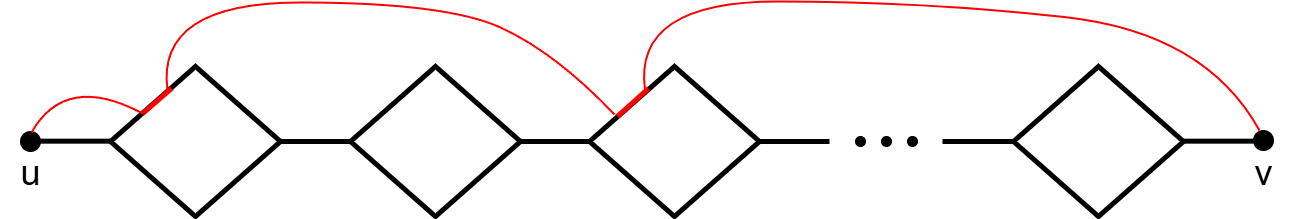
\includegraphics[width=120mm]{figures/chain_threads.png}   
    \label{fig:general_square_graph_pic}


    \begin{itemize}
    \item Chain link
    \begin{itemize}
        \item Initialization chain link
        \item Terminal chain link
        \item Literal chain link
    \end{itemize}
        \item Thread 
        \begin{itemize}
            \item 2-synchronization thread
            \item 3-synchronization thread
            \item Clause thread
        \end{itemize}
    \end{itemize}
\end{figure}
    
\end{frame}



\begin{frame}{Reduction from \textsc{3-SAT} to \textsc{Separating Shortest Path}}
\vspace{-1.8em}
\begin{algorithm}[H]
\tiny
\caption{Reduction from \textsc{3-SAT} to \textsc{Separating Shortest Path}}
\label{alg:reduction}
\begin{algorithmic}[1]
\Require Variables $X=\{x_1,\dots,x_n\}$, clauses $C=\{C_1,\dots,C_m\}$
\Ensure Graph $G$, vertices $u,v$
\State $n \gets |X|$, $m \gets |C|$
\State $G \gets \textsc{BuildChain}(u,v,2n+3m)$
\State $\mathcal{M} \gets$ map variable $\to$ list of literals
\For{$i \gets 1$ to $n$}
    \State $Lits \gets \mathcal{M}[x_i]$
    \State reserve $2+|Lits|$ chain links
    \State label first as $I_i$, last as $T_i$
    \For{each $\ell \in Lits$}
        \State assign next free link as $L_{\ell[0],\ell[1],i}$
    \EndFor
\EndFor
\For{$i \gets 1$ to $n$}
    \State $\textsc{Thread}(u,v,[(I_i,+),(T_i,-)])$
    \State $\textsc{Thread}(u,v,[(I_i,-),(T_i,+)])$
    \State $Lits \gets \mathcal{M}[x_i]$
    \For{each $\ell \in Lits$}
        \State $\textsc{Thread}(u,v,[(I_i,+),(L_{\ell[0],\ell[1],i},-),(T_i,+)])$
        \State $\textsc{Thread}(u,v,[(I_i,-),(L_{\ell[0],\ell[1],i},+),(T_i,-)])$
    \EndFor
\EndFor
\For{$i \gets 1$ to $m$}
    \State $\ell_1,\ell_2,\ell_3 \gets C_i$
    \State $\textsc{Thread}(u,v,[(L_{\ell_1[0],\ell_1[1]},s(\ell_1)),(L_{\ell_2[0],\ell_2[1]},s(\ell_2)),(L_{\ell_3[0],\ell_3[1]},s(\ell_3))])$
\EndFor
\State \Return $G$
\end{algorithmic}
\end{algorithm}
\end{frame}

\begin{frame}{Min Cut-Path Problem in Special Graph Classes}
\begin{thm}
Let \(G = (V, E)\) be a connected graph with diameter 2, and let \(u, v \in V\) be two distinct vertices. Then, the value of the min cut-path between \(u\) and \(v\) satisfies the following:
\[
cp(u, v) = c(u, v) + d(u, v) - 1.
\]
\end{thm}

\begin{thm}
\label{thm:min_cut_path_max_2}
Let \(G = (V, E)\) be a connected graph such that for every pair of distinct vertices \(x, y \in V\), the minimum cut satisfies:  
\[
c(x, y) \leq 2.
\]  
Then, the value of the min cut-path problem between \(u\) and \(v\) satisfies:
\[
cp(u, v) = c(u, v) + d(u, v) - 1.
\]
\end{thm}

\end{frame}

\section{$2^{nd}$ article}

\begin{frame}{$2^{nd}$ article}
\begin{itemize}
    \item \textbf{Motivation}
    \begin{itemize}
        \item Direct continuation of the first article
        \item Aims to unify previously identified polynomial-time islands
    \end{itemize}

    \item \textbf{Main focus}
    \begin{itemize}
        \item A unified polynomial-time class: \emph{diameter two or minimum cut-value two}
        \item Denoted as the \textbf{Diam-or-Cut-2} graph class
    \end{itemize}

    \item \textbf{Main contribution and methodology}
    \begin{itemize}
        \item Introduction of a \emph{general square graph decomposition}
        \item Structural characterization of the \textbf{Diam-or-Cut-2} class via this decomposition
        \item Design of a polynomial-time algorithm that, using the decomposition,
              decides the Min Cut-Path problem
    \end{itemize}

    \vspace{0.3cm}
    \item \textbf{Current status}
    \begin{itemize}
        \item The article is planned but not yet written
    \end{itemize}
\end{itemize}
\end{frame}


\begin{frame}{Diam or Cut 2 Graph}
\begin{defn}[Diam or Cut 2 Graph]
Let \(G = (V, E)\) be a graph. We say that \(G\) has the \textbf{diam or cut 2 graph} property if for every pair of distinct vertices \(x, y \in V\), at least one of the following conditions satisfies:
\[
c(x, y) \leq 2 \quad \text{or} \quad d(x, y) \leq 2.
\]  
\end{defn}
\begin{figure}[H]
    \centering
    \begin{minipage}{0.45\textwidth}
        \centering
        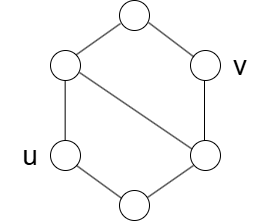
\includegraphics[width=35mm]{example_cut2.png}
        \subcaption{\textbf{\( c(u,v) = 2 \)}}
        \label{fig:example_cut2}
    \end{minipage}
    \hfill
    \begin{minipage}{0.45\textwidth}
        \centering
        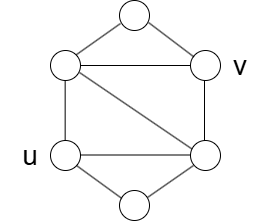
\includegraphics[width=35mm]{example_diam2.png}
        \subcaption{\textbf{\( d(u,v) = 2 \)}}
        \label{fig:example_diam2}
    \end{minipage}
    \caption{\textbf{Counterexample \( cp(u, v) \neq d(u, v) + c(u, v) - 1 \) }}
\end{figure}

\end{frame}

\begin{frame}{General Square Graph}
    \begin{figure}[H]
    \centering
    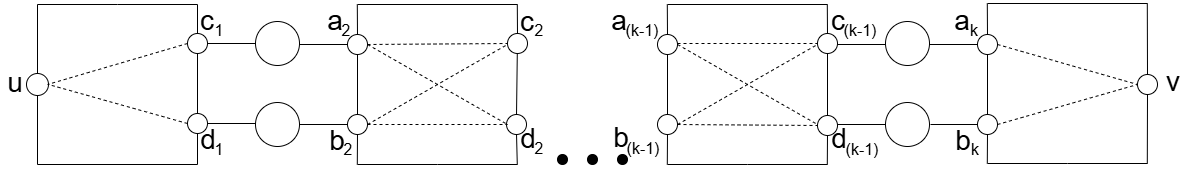
\includegraphics[width=120mm]{general_square_graph.png}   
    \label{fig:general_square_graph_pic}
\end{figure}
\end{frame}

\begin{frame}{Transformations}
\vspace{-0.8em}
\begin{figure}[H]
    \centering
    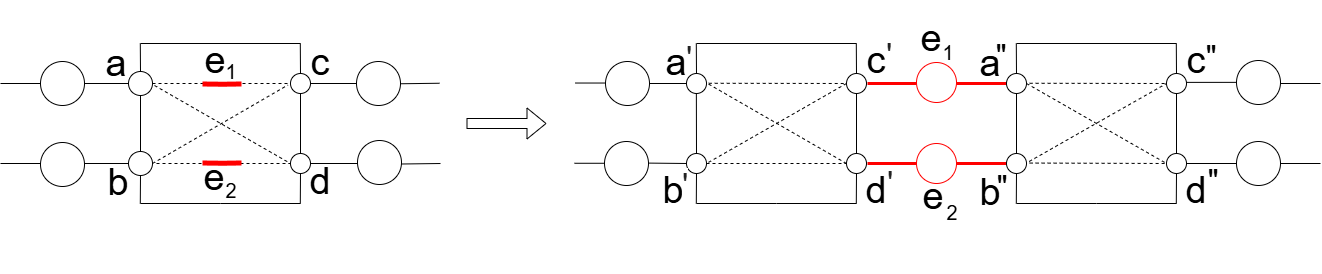
\includegraphics[width=120mm]{Transformation_A.png}
    \label{fig:Transformation_A}
\end{figure}

\vspace{-2.8em}
\begin{figure}[H]
    \centering
    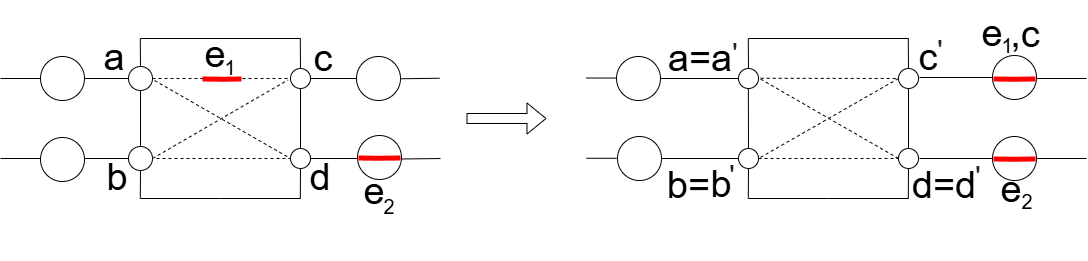
\includegraphics[width=100mm]{Transformation_B.png}
    \label{fig:Transformation_B}
\end{figure}

\vspace{-0.8em}
\begin{figure}[H]
    \centering
    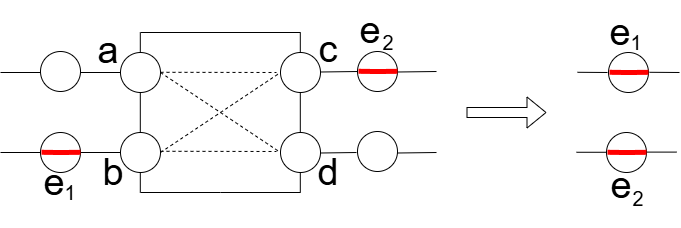
\includegraphics[width=70mm]{Transformation_C.png}
    \label{fig:Transformation_C}
\end{figure}
    
\end{frame}








\begin{frame}{Constructing a General Square Graph Decomposition}
\vspace{-1em} 
\begin{algorithm}[H]
\tiny
\label{alg:square_graph_revised}
\begin{algorithmic}[1]
\Require Graph \(G=(V,E)\) with property diam or cut 2, vertices \(u,v \in V\) such that \(c(u,v)=2\)
\Ensure A decomposition G into a valid square general graph between \(u\) and \(v\).

\State Initialize pseudo-square graph \(S_{initial}\) with \(a=u, b=u, c=v, d=v\) and \(V=V(G)\).
\State \(e_1, e_2 \leftarrow\) min \(cut(u, v)\)
\State \(S'_1, S'_2 \leftarrow\) TransformationA(\(G,S_{initial},e_1, e_2,u,v\)). 
\State Initialize \(S \leftarrow \{S'_1, S'_2\}\).

\While{\(S\) is not empty}
    \State \(S_{work} \leftarrow\) select and remove pseudo-square graph from \(S\).
    \For{each pair \((x, y)\) in \(\{(a, c), (b, d), (a, d), (b, c)\}\)}
        \If{\(d(x, y) > 2\)} \Comment{Checking if a pseudo-square graph is a square graph}
            \State \(e_1, e_2 \leftarrow\) min \(cut(x, y)\) \Comment{Edges \(e_1\) and \(e_2\) are within \(S_{work}\) intesection general paths that connects to this pseudo-square graph.}
            \State \(Count \leftarrow count(e_1, e_2 \in S_{work})\)
            \Switch{\(Count\)}
                \Case{0}
                    \State TransformationC(\(G,S_{work},e_1, e_2,x,y\))
                \EndCase
                \Case{1}
                    \State \(S'_1 \leftarrow\) TransformationB(\(G,S_{work},e_1, e_2,x,y\))
                    \State Add \(S'_1\) to \(S\).
                \EndCase
                \Case{2}
                    \State \(S'_1, S'_2 \leftarrow\) TransformationA(\(G,S_{work},e_1, e_2,x,y\))
                    \State Add \(S'_1, S'_2\) to \(S\).
                \EndCase
            \EndSwitch
            \State \textbf{break}
        \EndIf 
    \EndFor
\EndWhile
\State \textbf{Return} the constructed general square graph.
\end{algorithmic}
\end{algorithm}
    
\end{frame}

\begin{frame}{General Square Graph}
    \begin{figure}[H]
    \centering
    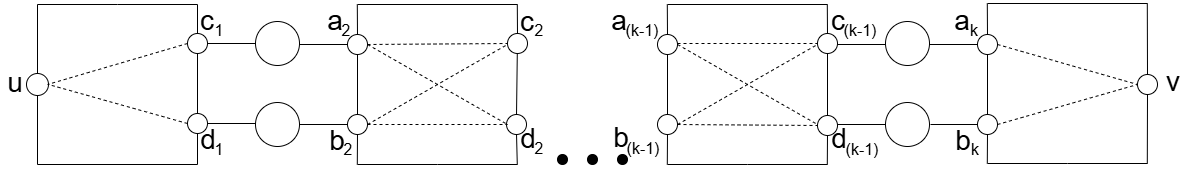
\includegraphics[width=120mm]{general_square_graph.png}   
    \label{fig:general_square_graph_pic}
\end{figure}
\end{frame}

\begin{frame}{Polynomial-time algorithm}
\vspace{-1em}
    \begin{algorithm}[H]
    \tiny
\caption{Polynomial-time algorithm for computing \(cp(u,v)\) in a graph with the \textbf{diam or cut 2} property and \(c(u,v) = 2\)}
\begin{algorithmic}[1]
\Require Graph \(G=(V,E)\) with property diam or cut 2, vertices \(u,v \in V\) such that \(c(u,v)=2\)
\Ensure Value of \(cp(u,v)\)

\State Compute \(d(u,v)\) using breadth-first search
\State Construct the \textit{general square graph} \(H\) from \(G\) on vertices \(u,v\)
\State \(S \gets \emptyset\)
\ForAll{square graphs \(S_i\) in \(H\)}
    \State \(S \gets S \cup \{S_i\}\)
\EndFor

\ForAll{\(S_i \in S\)}
    \ForAll{possible vertex pairs \((x,y)\) as per Definition~\ref{defn:square_graph}}
        \State \(\{\alpha, \beta\} \gets\) the remaining two vertices of \(S_i\)
        \State \(P \gets\) the set of all shortest paths \(\leq2\) between \(x\) and \(y\)\Comment{We compute the shortest path within the square graph \(S_i\).}
        \ForAll{\(p \in P\)}
            \If{\(\alpha\) and \(\beta\) are in different components after removing the edges of path \(p\)}
                \State \(res \gets d(u,x) + d(x,y) + d(y,v)\)
                \If{\(res = d(u,v)\)}
                    \State \Return \(d(u,v)\)
                \EndIf
            \EndIf
        \EndFor
    \EndFor
\EndFor
\State \Return \(d(u,v) + 1\)
\end{algorithmic}
\end{algorithm}
\end{frame}

\begin{frame}{Linear-time algorithm (1/2)}
    \begin{algorithm}[H]
    \tiny
\caption{Linear-time algorithm for computing \(cp(u,v)\) in a graph with the \textbf{diam or cut 2} property and \(H\) as a general square graph}
\begin{algorithmic}[1]
\Require Graph \(G=(V,E)\), vertices \(u,v \in V\), general square graph \(H\)
\Ensure Value of \(cp(u,v)\)

\State Compute \(d(u,v)\) using BFS


\State \(S \gets \emptyset\)
\ForAll{square graphs \(S_i\) in \(H\)}
    \State \(S \gets S \cup \{S_i\}\)
\EndFor

\State Compute distance tables \(D_1, D_2\) using dynamic programming, where:
\begin{itemize}
    \item \(D_1[x]\) stores \(d(u,x)\) for all \(x \in  G\)
    \item \(D_2[x]\) stores \(d(x,v)\) for all \(x \in G\)
\end{itemize}
\end{algorithmic}
\end{algorithm}
\end{frame}
\begin{frame}{Linear-time algorithm (2/2)}
    \begin{algorithm}[H]
    \tiny
\caption{Linear-time algorithm for computing \(cp(u,v)\) in a graph with the \textbf{diam or cut 2} property and \(H\) as a general square graph}
\begin{algorithmic}[1]
\ForAll{\(S_i \in S\)}
    \ForAll{possible vertex pairs \((x,y)\) as per Definition~\ref{defn:square_graph}}
        \State \(\{\alpha, \beta\} \gets\) the remaining two vertices of \(S_i\)
        \State \(P \gets \emptyset\) 


      \State \( P \leftarrow P\) \(\cap \) \text{last edge of path} \( \alpha \text{ and } x \)
      \State \( P \leftarrow P\) \(\cap \) \text{last edge of path} \( \alpha \text{ and } y \)
      \State \( P \leftarrow P\) \(\cap \) \text{last edge of path} \(\beta \text{ and } x \)
      \State \( P \leftarrow P\) \(\cap \) \text{last edge of path} \( \beta \text{ and } y \)

        \If{the shortest path distance from \(x\) to \(y\) is \(\leq 1\)}
            \State \(P \gets\) the unique shortest path
        \Else
            \State Ensure all partial paths in \(P\) are of length 2; if not, remove edges violating this.
        \EndIf

        \ForAll{\(p \in P\)}
            \If{\(\alpha\) and \(\beta\) are in different components after removing the vertices of path \(p\)}
                \State \(res \gets D_1[x] + d(x,y) + D_2[y]\)
                \If{\(res = d(u,v)\)}
                    \State \Return \(res\)
                \EndIf
            \EndIf
        \EndFor
    \EndFor
\EndFor
\State \Return \(d(u,v) + 1\)
\end{algorithmic}
\end{algorithm}
\end{frame}

\section{Teaching Activities}
\begin{frame}{Teaching Activities}
\vspace{-0.6em}
\begin{itemize}
    \item course: Project in Data Analysis II
    \item format: exercises only
    \item main goal: investment portfolio creation
    \item core topics:
    \begin{itemize}
        \item stock buy/sell indicators
        \item technical analysis
        \item neural networks
    \end{itemize}
    \item final output:
    \begin{itemize}
        \item trading bot
        \item historical market data
        \item real-time market data
        \item performance optimization
    \end{itemize}
\end{itemize}
\end{frame}
\section{Supervision and Consulting}
\begin{frame}{Supervision and Consulting}
\vspace{-0.6em}
\begin{itemize}
    \item role: consultant
    \item bachelor thesis
    \item student: Tomáš Oltman
    \item topic: Chess Engine
    \item focus: decision-making strategies
    \item techniques:
    \begin{itemize}
        \item reinforcement learning
        \item heuristic evaluation
        \item search-based methods
    \end{itemize}
\end{itemize}

\end{frame}

\section{Future Plans}
\begin{frame}{Future Plans}
\vspace{-0.6em}
\begin{itemize}
    \item completion of the second paper
    \item application of graph neural networks to:
    \begin{itemize}
        \item Min Cut-Path
        \item Traveling Salesman Problem
    \end{itemize}
    \item design of new algorithms and analysis of their approximation properties
    \item algorithm development for specific datasets
    \item study of approximation algorithms for stochastic variants of the Vehicle Routing Problem
\end{itemize}
\end{frame}

\section{Support with Activities}
\begin{frame}{Support with Activities}
\vspace{-0.6em}
\begin{itemize}
    \item \textbf{Kapustnica} (traditional Slovak cabbage soup)
    
    \item \textbf{ASEF}
    \begin{itemize}
        \item Two terms: 2--5 December and 4--6 November
    \end{itemize}
    
    \item \textbf{Technical assistance}
\end{itemize}
\end{frame}


\begin{frame}{Thank You}
\vspace{1.5em}
\begin{center}
    \Large Thank you for your attention
\end{center}
\end{frame}










\end{document}
